\subsection{Supporting Technology}
\label{sub:sec:SERAFramework}

In the research community there are several frameworks to ease the development of virtual agents in \ac{HRI} by promoting reusability between components. Examples of frameworks include SEMAINE~\cite{Schroder2010a}, \acl{VHT}~\cite{Hartholt2013}, \acl{ASAP}~\cite{Kopp2013}, Robot Behaviour Toolkit~\cite{Huang2012}, and \ac{SERA}~\cite{Tullio2015}. The solution will choose the latter as it is being developed internally in \ac{GAIPS}, is used extensively in several \ac{HRI} studies~\cite{Tullio2015}, and was tested in several different embodied robots such as \ac{EMYS} (Figure~\ref{fig:robots:EMYS}) and Keepon (Figure~\ref{fig:robots:Keepon}).

%\vspace{-4mm}
\begin{figure}[ht]
	\begin{minipage}[b]{.4\textwidth}
		\centering
		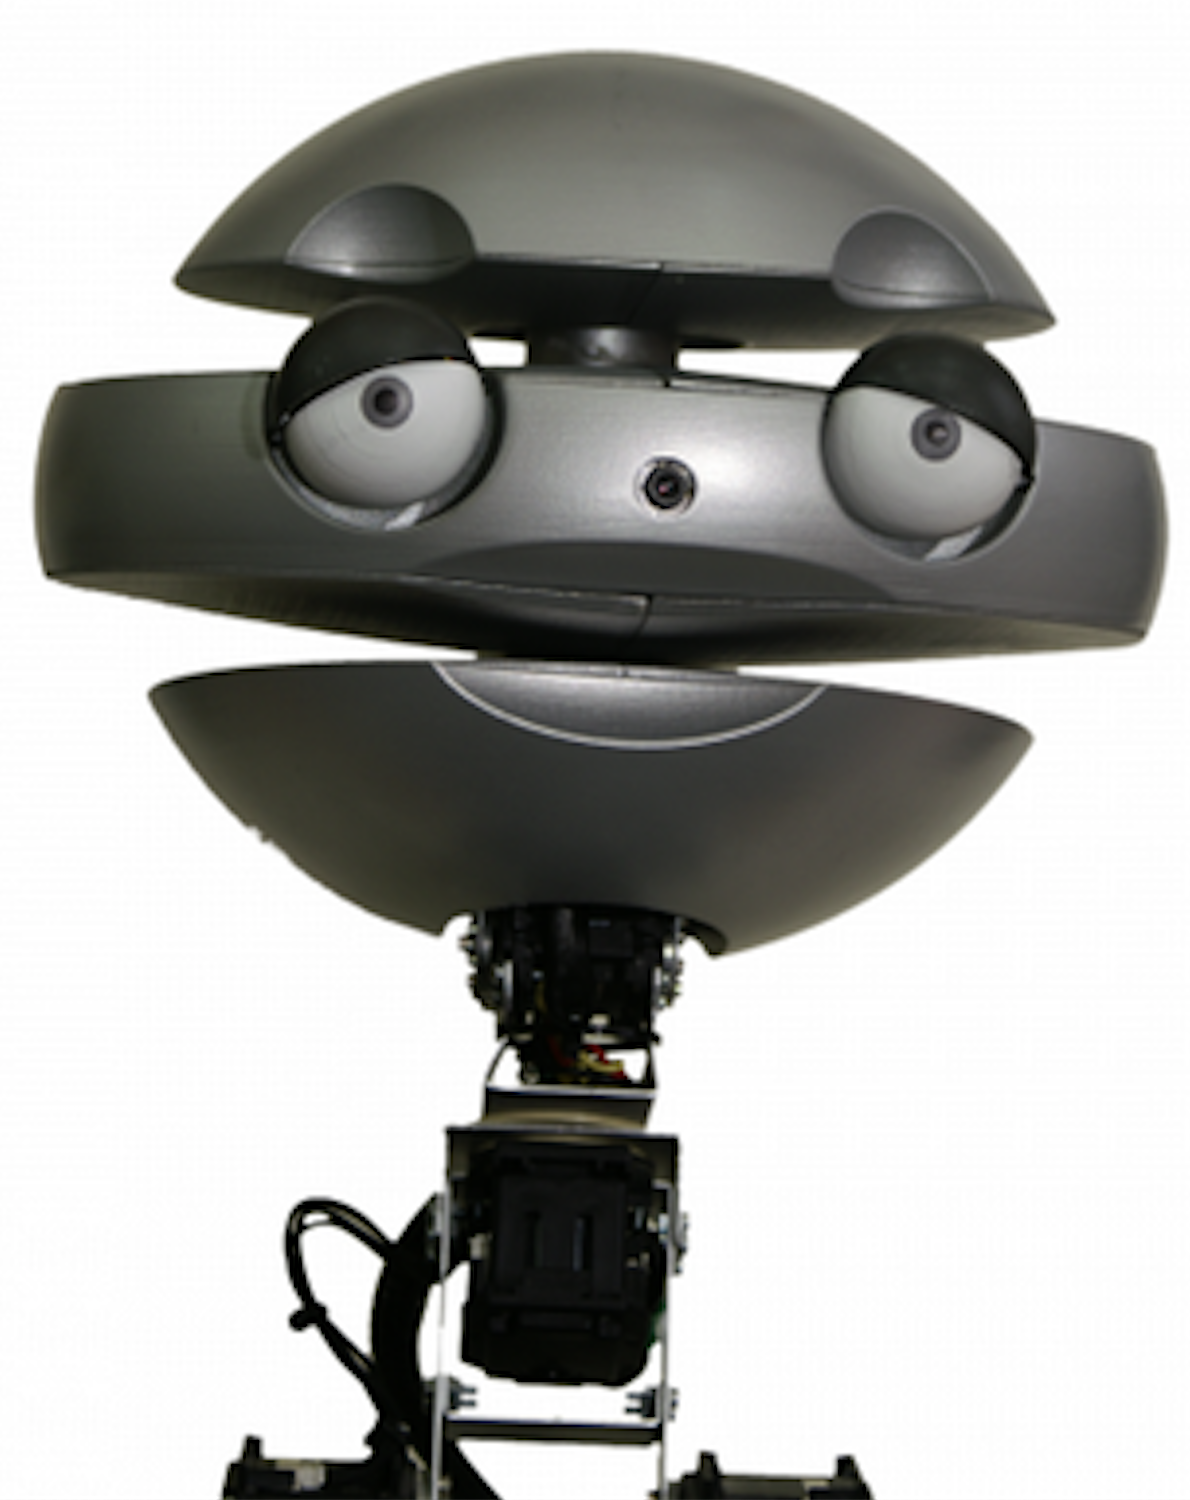
\includegraphics[width=0.4\textwidth]{images/emys.png}
		\caption{EMYS robot.}
		\label{fig:robots:EMYS}
	\end{minipage}
	\hfill
	\begin{minipage}[b]{.4\textwidth}
		\centering
		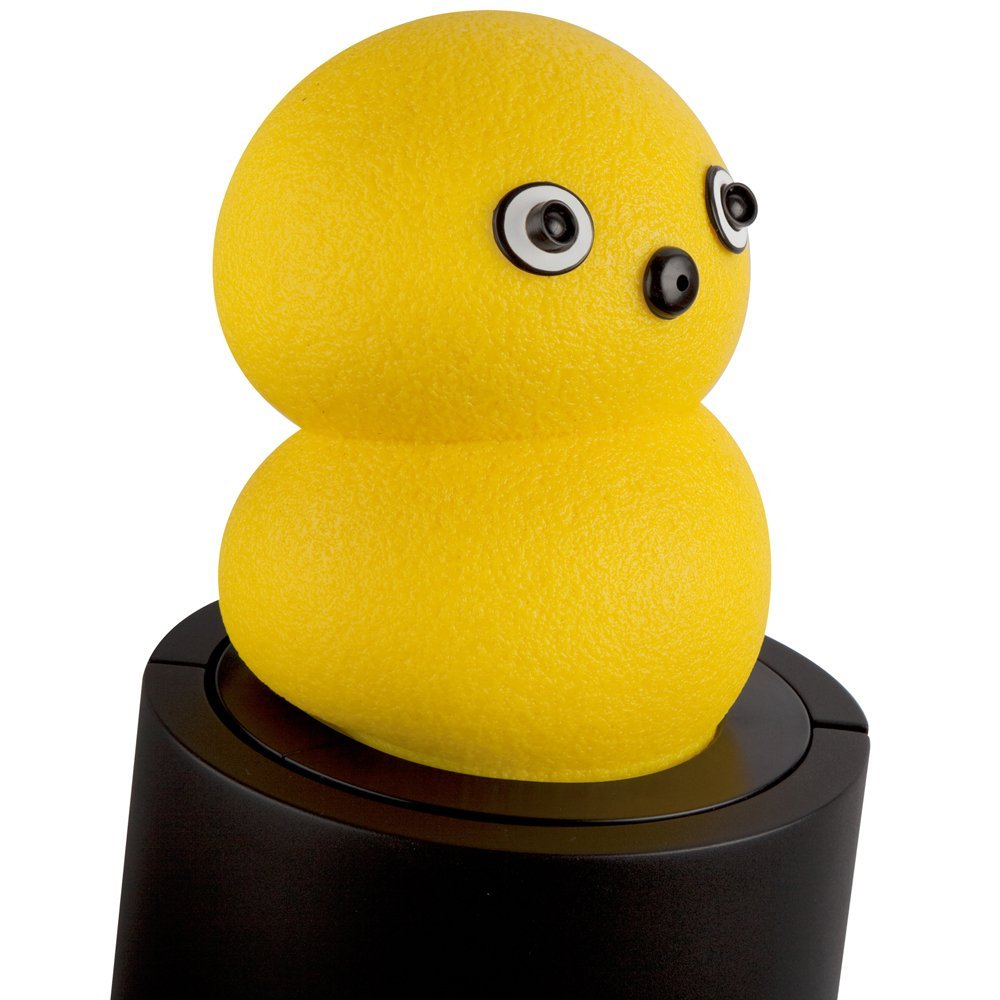
\includegraphics[width=0.4\textwidth]{images/Keepon.jpg}
		\caption{Keepon robot.}
		\label{fig:robots:Keepon}
	\end{minipage}
\end{figure}
%\vspace{-4mm}

\ac{SERA} follows the SAIBA model~\cite{Kopp2006} and is very similar to \ac{ROS}~\cite{Quigley2009} due to, respectively, the separation between intention planning, behaviour planning and realisation, and due to the usage of decoupled modules in an asynchronous messaging system. It aims to be used by both technical and non-technical developers such as psychologists~\cite{Tullio2015}, an advantage as their knowledge is crucial during the development and analysis of \ac{HRI}. For example, utterances are modelled using markup text that can contain non-interrupting behavioural rules and can be developed by non-technical teams.

The most important components are Thalamus, Skene and Nutty Tracks.
\begin{itemize}
	\item \textbf{\textit{Thalamus}}: responsible for receiving and delivering the published messages to the right subscribers;
	\item \textbf{\textit{Skene}}: responsible for translating high-level intentions generated at the decision-making level into a schedule of behaviour actions;
	\item \textbf{\textit{Nutty Tracks}}: responsible for managing animations.
\end{itemize}

\textit{Skene} is the most relevant component in \ac{SERA} for the development of rapport agents as it is the controller that plans animations and non-verbal behaviours such as gaze, utterances and animations according to perceptual messages. This component is rule-based and has an explicit representation of its body position over his physical environment. 

SERA also includes modules for bridging external tools such as \ac{FAtiMA} to model emotions~\cite{Dias2011} or Unity to create virtual scenarios. All these modules co-exist inside the \textit{Thalamus} ``network'' to cooperate, in order to achieve the interactional goals in any \ac{HRI} scenario (e.g., negotiation scenarios on Figure~\ref{fig:SERA:Examples}).

\begin{figure}
	\centering
	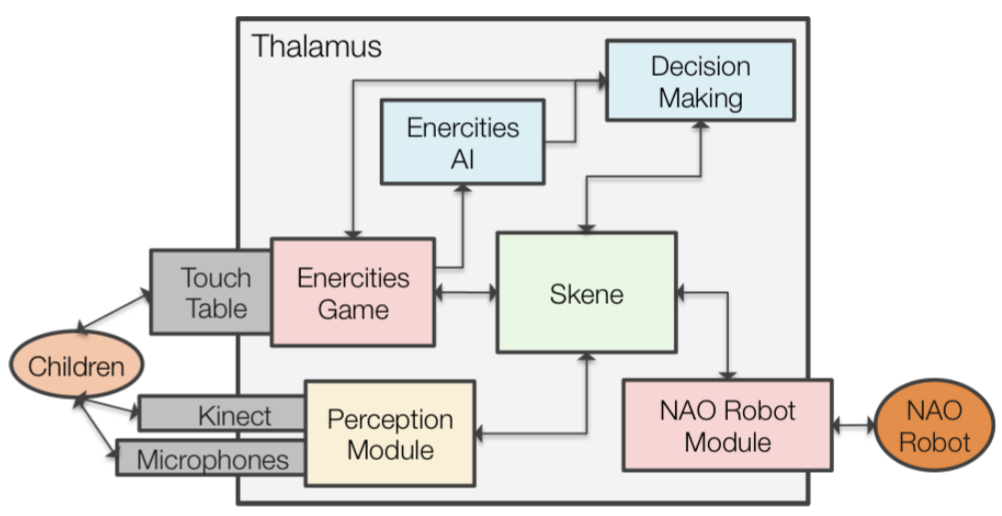
\includegraphics[width=0.6\linewidth]{images/SERA_ExSystemEC.png}
	\caption{Enercities scenario system architecture integrated with SERA framework. From~\cite{Tullio2015}.}
	\label{fig:SERA:Examples}
\end{figure}
%\vspace{-4mm}

Despite being under development, \ac{SERA} is stable and demonstrates its applicability in a wide range of \ac{HRI} scenarios. However, the \textit{Skene} component lacks rapport management strategies and it does not adapt its actions when interrupted by the user, which reduces coordination and the overall feeling of rapport. Moreover, the \textit{Skene} component is rule-based which is not sufficiently elegant to build systems more appealing and natural to end-users.